\documentclass[notitlepage]{report}

\title{
	\textsc{ \small
		Physics 415
	} \\
	{\textsc{\small Lab \#7}} \\
	Gamma Ray Spectroscopy
}
\author{Kevin Evans \\ Partner: Sierra Ray}
\date{April 20, 2021}
\usepackage{amssymb}
\usepackage{mathtools}

\usepackage{amsthm}
\usepackage{amsmath}
\usepackage{slashed}
\usepackage{relsize}
\usepackage{threeparttable}
\usepackage{float}
\usepackage{booktabs}
\usepackage{boldline}
\usepackage{changepage}
\usepackage{physics}
\usepackage[inter-unit-product =\cdot]{siunitx}
\usepackage{setspace}
\usepackage{caption}
\usepackage{subcaption}
\usepackage[makeroom]{cancel}
%\usepackage{pgfplots}

\usepackage{enumitem}
\usepackage{times}
\usepackage{titling} % for titlingpage environment
\usepackage{calligra}
\usepackage{graphicx}
\DeclareMathAlphabet{\mathcalligra}{T1}{calligra}{m}{n}
\DeclareFontShape{T1}{calligra}{m}{n}{<->s*[2.2]callig15}{}
\newcommand{\scriptr}{\mathcalligra{r}\,}
\newcommand{\boldscriptr}{\pmb{\mathcalligra{r}}\,}
\newcommand{\emf}{\mathcal{E}}
\renewcommand{\thesection}{\arabic{section}}

\begin{document}
	\begin{titlingpage}
		\maketitle
		\begin{abstract}
			\noindent In this experiment, a scintillation counter was used to monitor the decay of several decaying isotopes: Sodium-22, Manganese-54, Cesium-137, Cobalt-60, Cadmium-107, and Barium-138. Additionally, Cobalt-57 was analyzed but was found to have a weak decay and no features were observed in its spectrum.
			A calibration curve was found using the photopeak energies. Using the backscattering energy, the electron mass was found to be \SI{509.656}{\keV}, at 0.2\% error of the accepted value. The energy resolution of the detector was found to be \SI{90.98}{\keV}.
		\end{abstract}
	\end{titlingpage}

	\section{Description of Experiment}
	Initially, the background radiation was measured using the scintillation counter. This was done by recording data of the empty lead chamber for roughly 300 seconds, then subtracting this background radiation from subsequent recordings.
	
	For each isotope sample, a spectrum was recorded exceeding 300 seconds and the background radiation was subtracted out. The photopeaks were identified using a Gaussian curve fit within Origin. The channels were recorded along with the expected energy. This data was plotted in Origin and a linear fit was applied, giving a mapping between channel number and energy.
	
	The corresponding features of the graphs were marked on the plots. On the Cesium-137 sample, the approximate Compton edge was identified and the mass of the electron was calculated from this decay. The mass of the electron can be found using \begin{align*}
		E_\gamma' & = \frac{E_\gamma}{1 + \frac{ E_\gamma }{m_e c^2} \left(1 - \cos\theta\right)}
	\end{align*}
	where $\gamma$ is the incident photon, $\gamma'$ is the backscattered photon. The backscattered photon energy can be determined from the plots, where $E_{\gamma'} = E_\gamma - E_e$. Then, this can be simplified as \begin{equation}
		E_\gamma - E_e = \frac{E_\gamma}{1 + \frac{2 E_\gamma}{m_e c^2}}. \label{eq:compton}
	\end{equation}
	The energy resolution of the detector can be found by analyzing the photopeak of Cesium-137. Here, we expect a sharp peak at the photo peak energy. By applying a Gaussian fit, we can find the full-width half-max value and take this as the energy resolution of the detector.
	\section{Data and Analysis}
	The photopeak energies for all but the Cobalt-57 spectrum were matched with their corresponding channel number and plotted in Figure \ref{fig:callibration}. Applying a linear fit with $R^2=$, the mapping between channel number and energy was found to be \begin{equation}
		E_n = -0.01842 + 0.00151 n \qquad [\si{\MeV}]
	\end{equation}
	where $n$ is the channel number. This was applied to all of the spectra plots, shown in Figure \ref{fig:na22} through \ref{fig:ba138} below. 
	
	By analyzing the Cesium-137 sample, the photopeak and approximate backscattering edge was found to have energies \SI{0.662}{\MeV} and \SI{0.478}{\MeV} respectively. Applying \eqref{eq:compton}, the electron mass was estimated $$m_e = \SI{509.656}{\keV}.$$ This is roughly 0.2\% error from the accepted \SI{511.0}{\keV}.
	
	The energy resolution can be found by the curve fit shown in Figure \ref{fig:cs137}. Here, the FWHM was found to be $2w = \SI{90.98}{\keV}$.
		
	
	\section{Results and Conclusion}
	 A scintillation counter was used to monitor the decay of several decaying isotopes: Sodium-22, Manganese-54, Cesium-137, Cobalt-60, Cadmium-107, and Barium-138. Additionally, Cobalt-57 was analyzed but was found to have a weak decay and no features were observed in its spectrum. This was likely due to a weak source or user error. It may be possible that the measured time was too short and additional features may improve with time.
	 
	 A calibration curve was found using the photopeak energies. Using the backscattering energy, the electron mass was found to be \SI{509.656}{\keV}, at 0.2\% error of the accepted value. The energy resolution of the detector was found to be \SI{90.98}{\keV}.
		
		
	\begin{figure}[p]
	\centering
	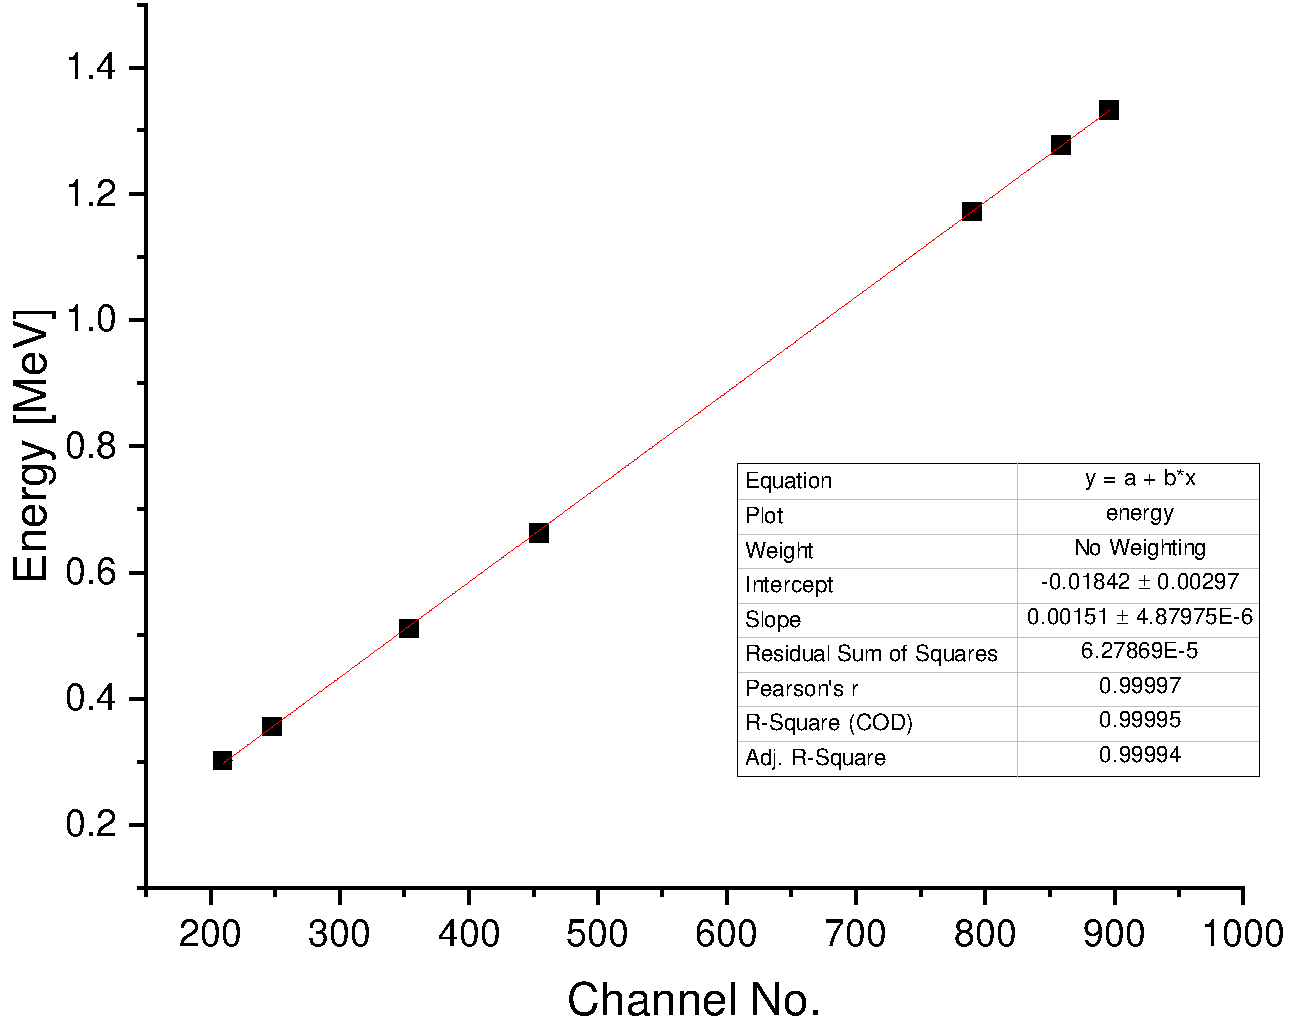
\includegraphics[width=0.7\linewidth]{callibration}
	\caption{Calibration curve; mapping the channel to energy.}
	\label{fig:callibration}
\end{figure}
\begin{figure}[p]
	\centering
	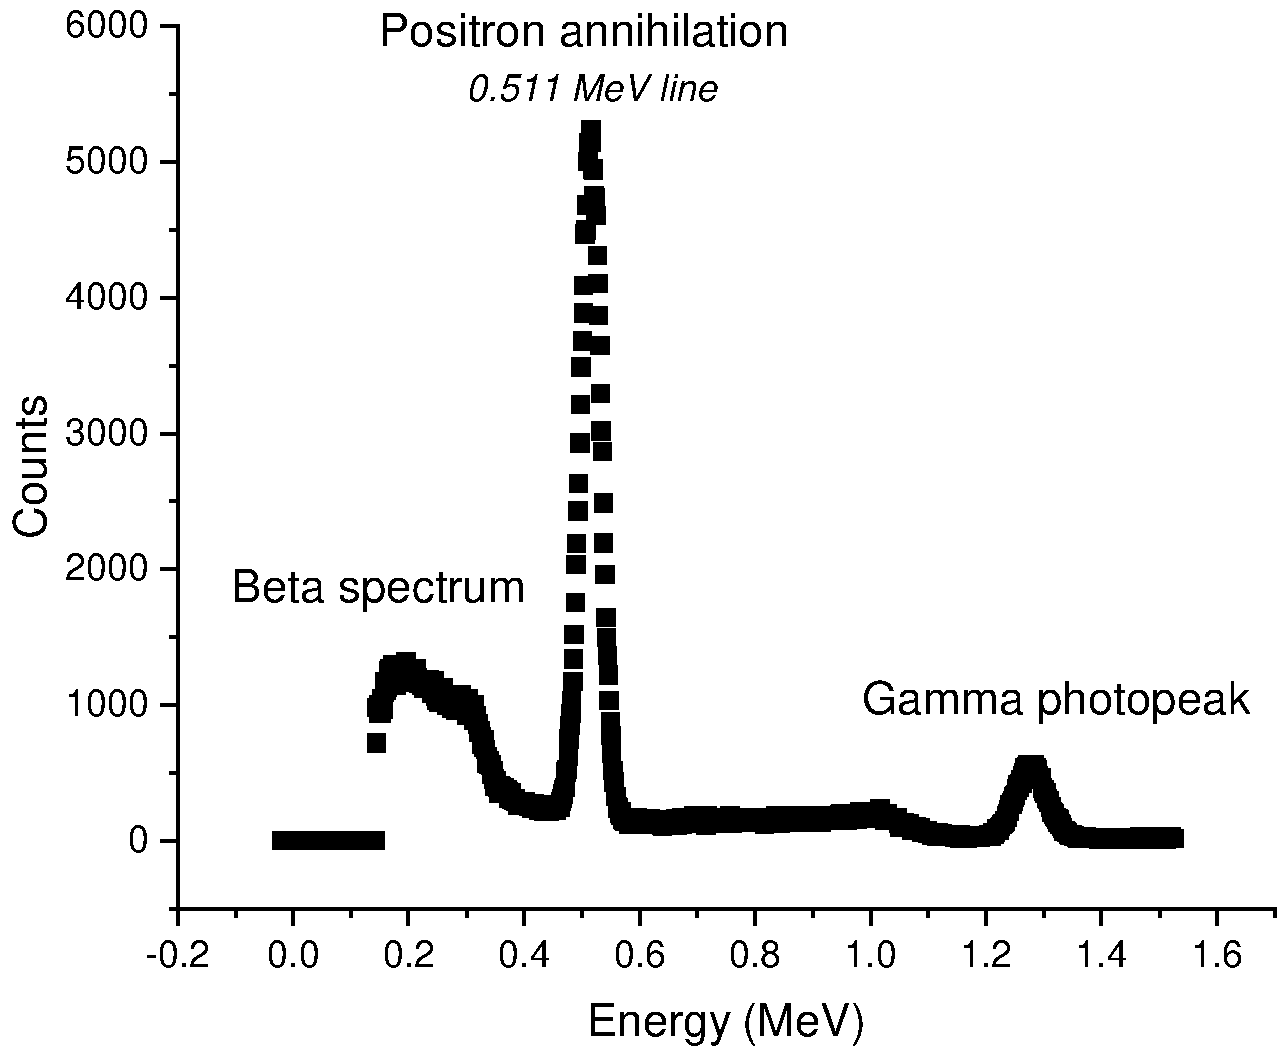
\includegraphics[width=0.7\linewidth]{na22}
	\caption{Sodium-22 spectrum, 611 seconds.}
	\label{fig:na22}
\end{figure}
\begin{figure}[p]
	\centering
	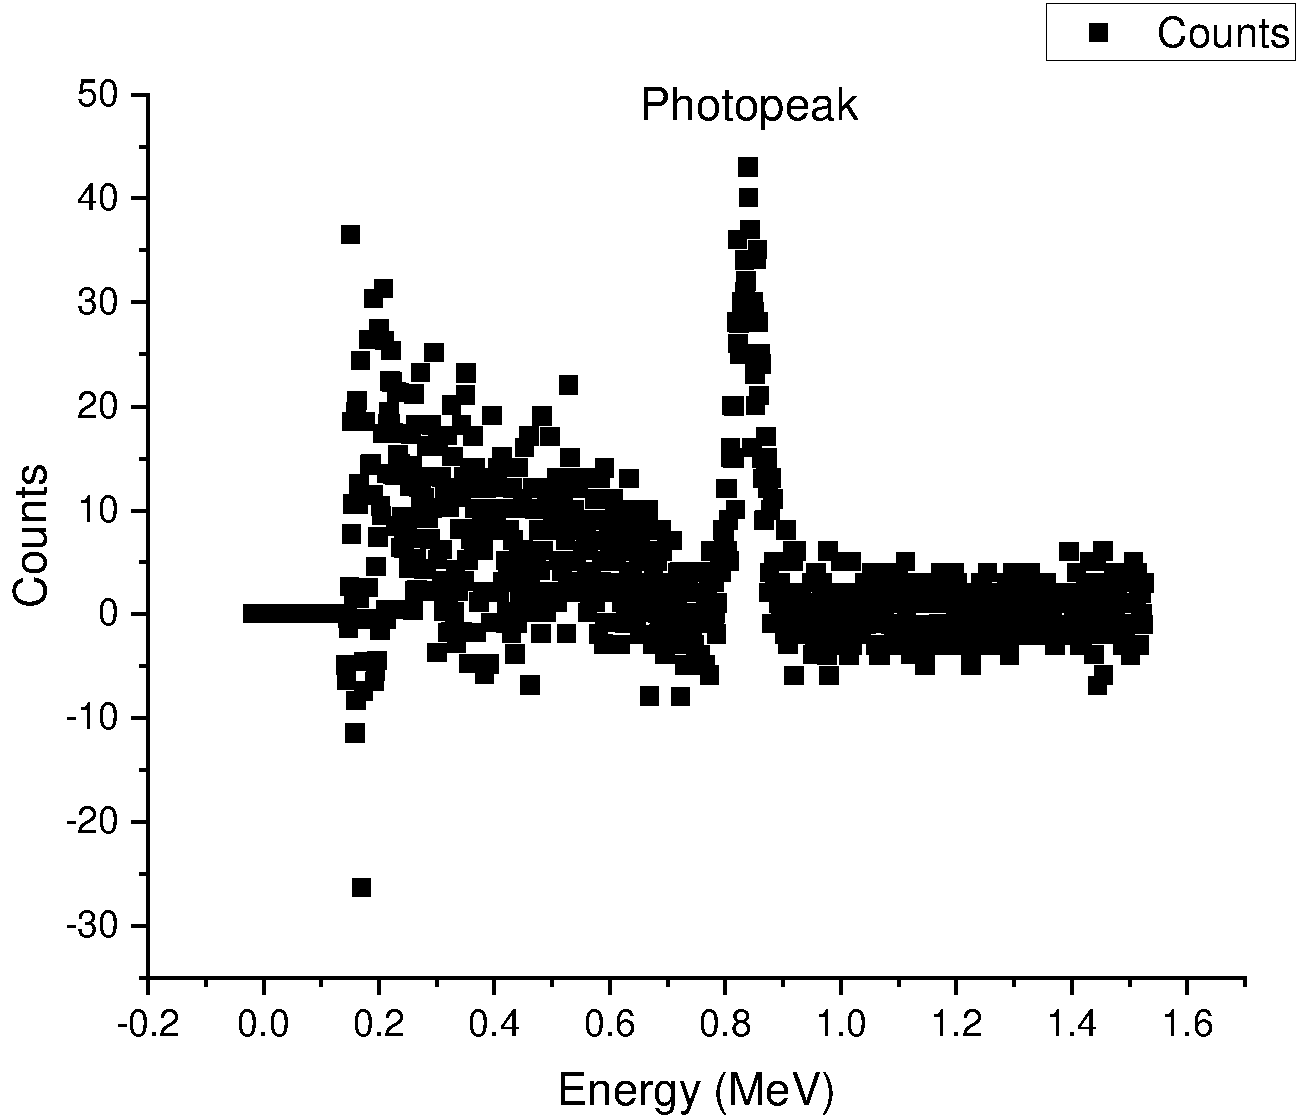
\includegraphics[width=0.7\linewidth]{mn54}
	\caption{Manganese-54 spectrum, 607 seconds.}
	\label{fig:mn54}
\end{figure}
\begin{figure}[p]
	\centering
	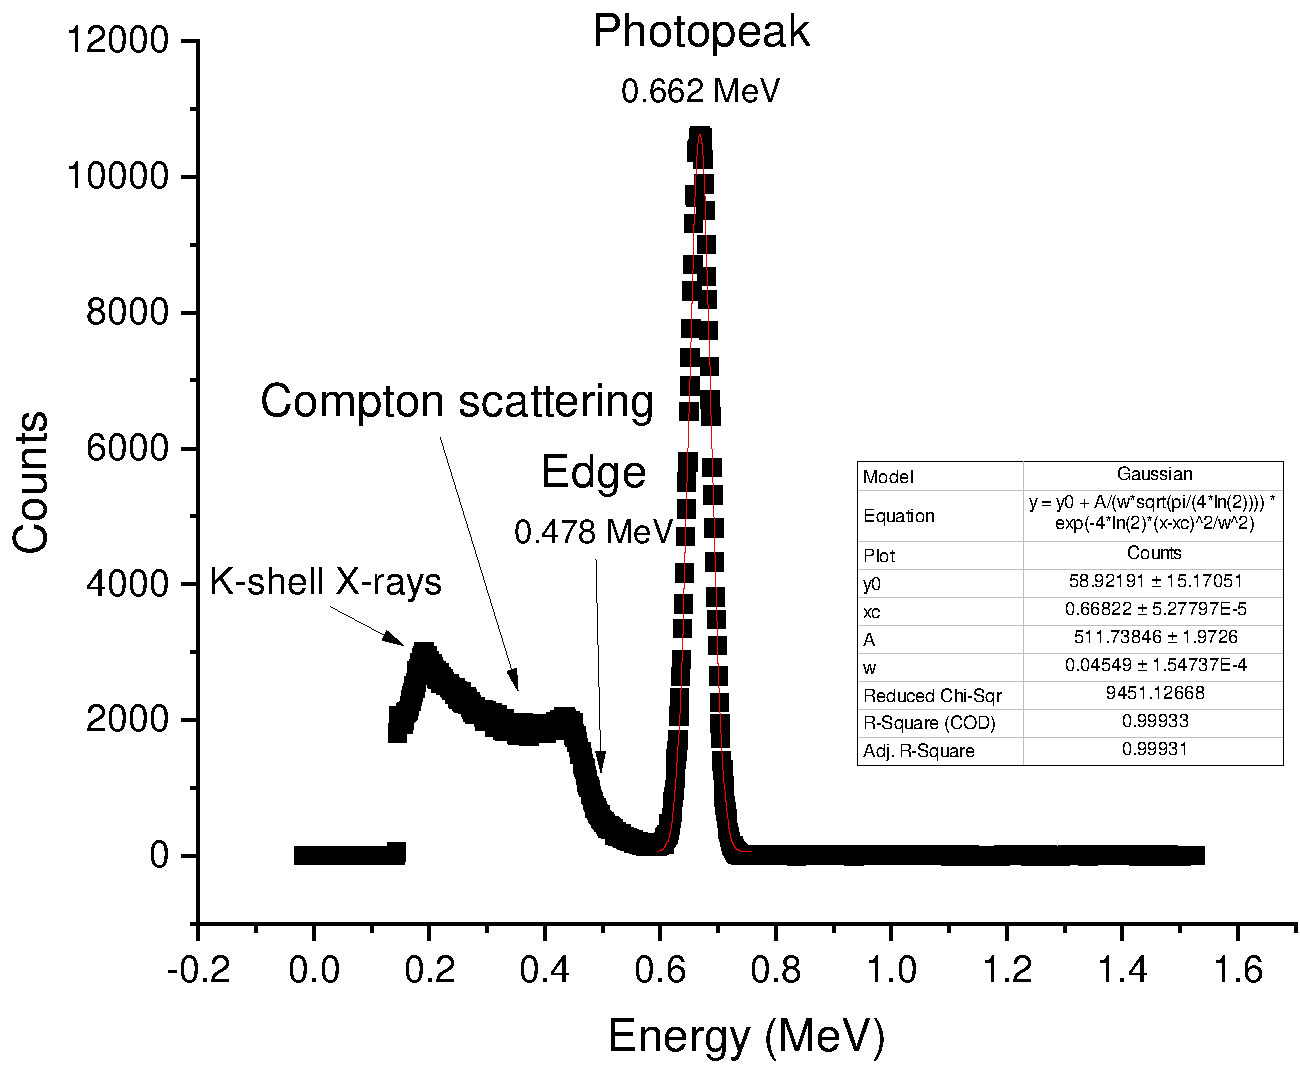
\includegraphics[width=0.7\linewidth]{cs137}
	\caption{Cesium-137 spectrum, 733 seconds. Included is a Gaussian fit at photopeak.}
	\label{fig:cs137}
\end{figure}
\begin{figure}[p]
	\centering
	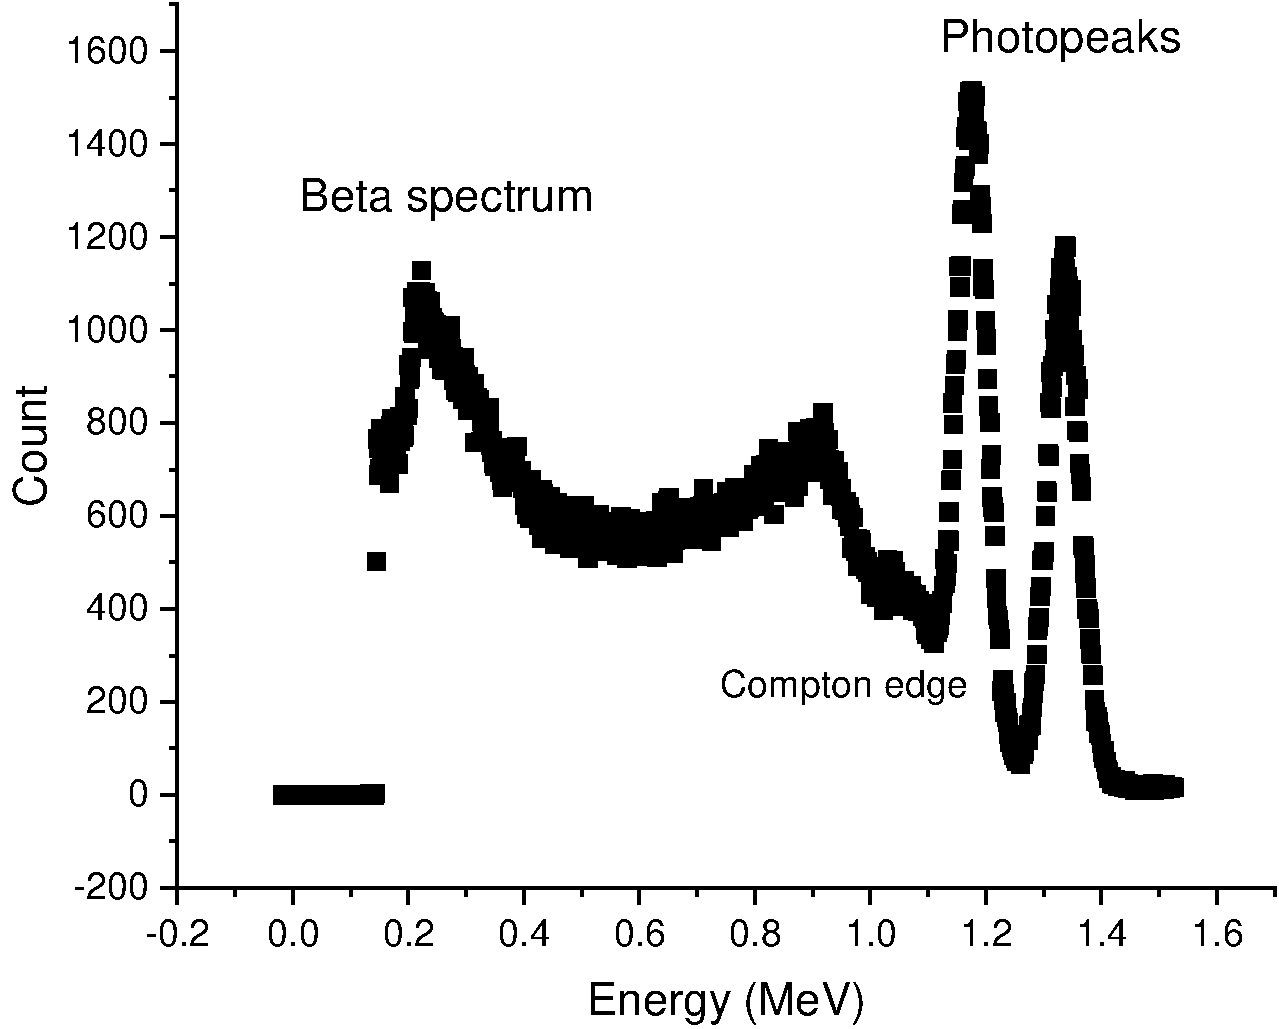
\includegraphics[width=0.7\linewidth]{co60}
	\caption{Cobalt-60 spectrum, 608 seconds.}
	\label{fig:co60}
\end{figure}
\begin{figure}[p]
	\centering
	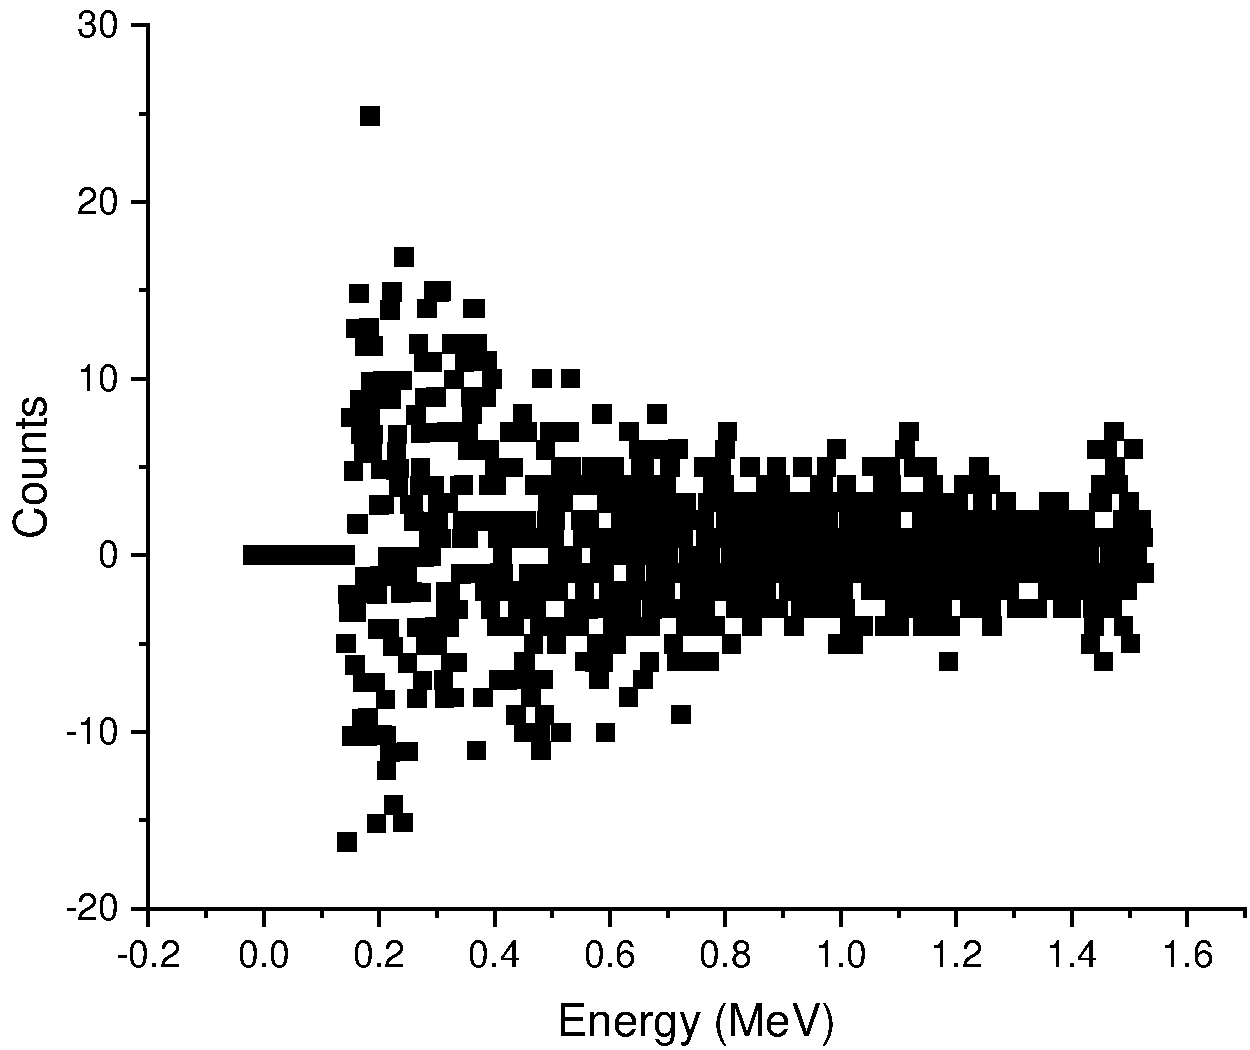
\includegraphics[width=0.7\linewidth]{co57}
	\caption{Cobalt-57 spectrum, 615 seconds.}
	\label{fig:co57}
\end{figure}
\begin{figure}[p]
	\centering
	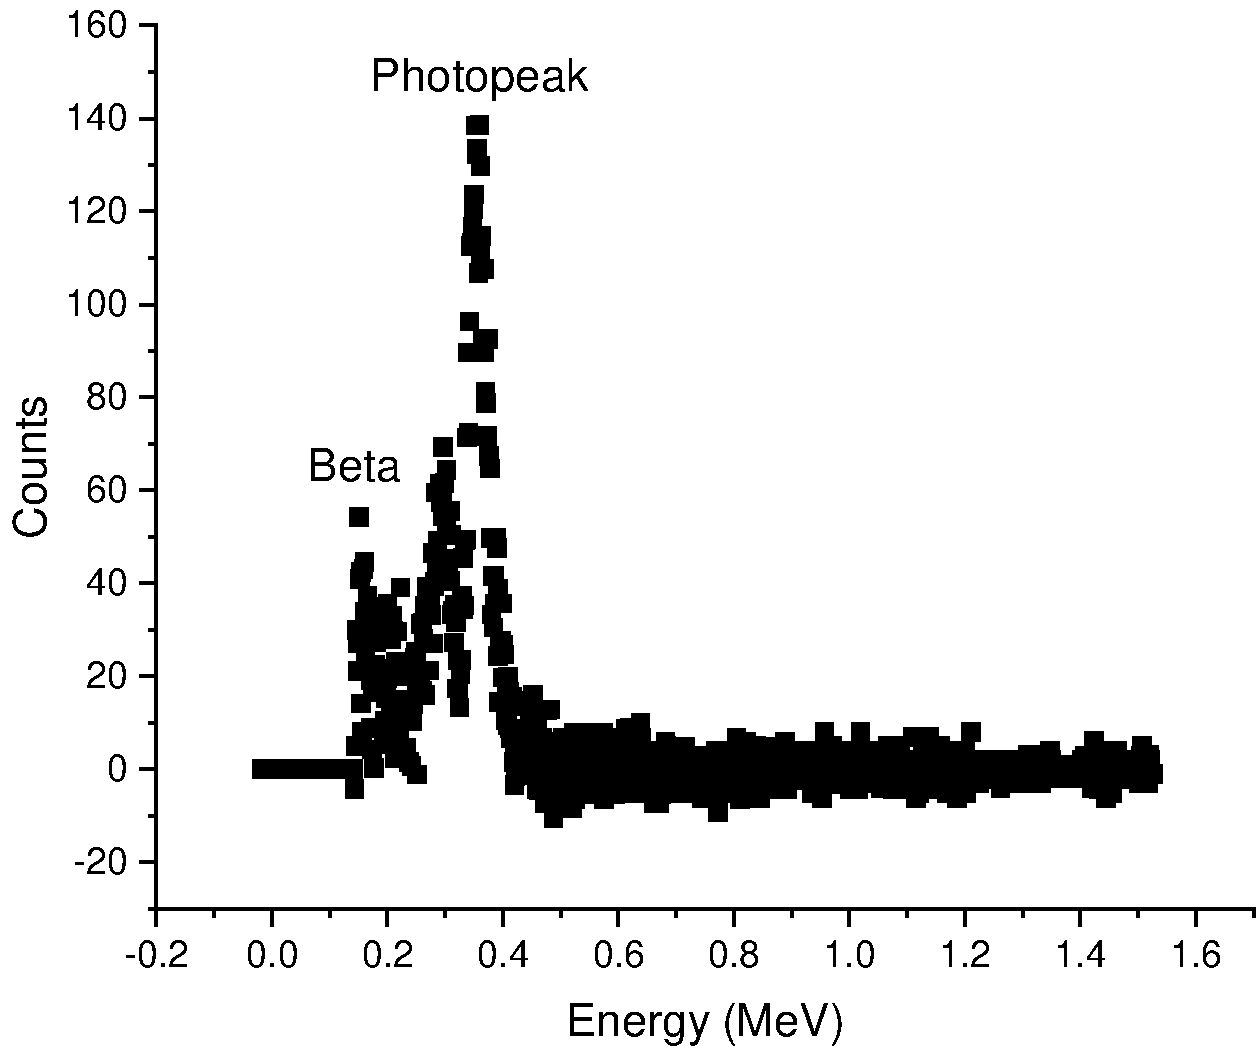
\includegraphics[width=0.7\linewidth]{cd107}
	\caption{Cadmium-107 spectrum, 632 seconds.}
	\label{fig:cd107}
\end{figure}
\begin{figure}[p]
	\centering
	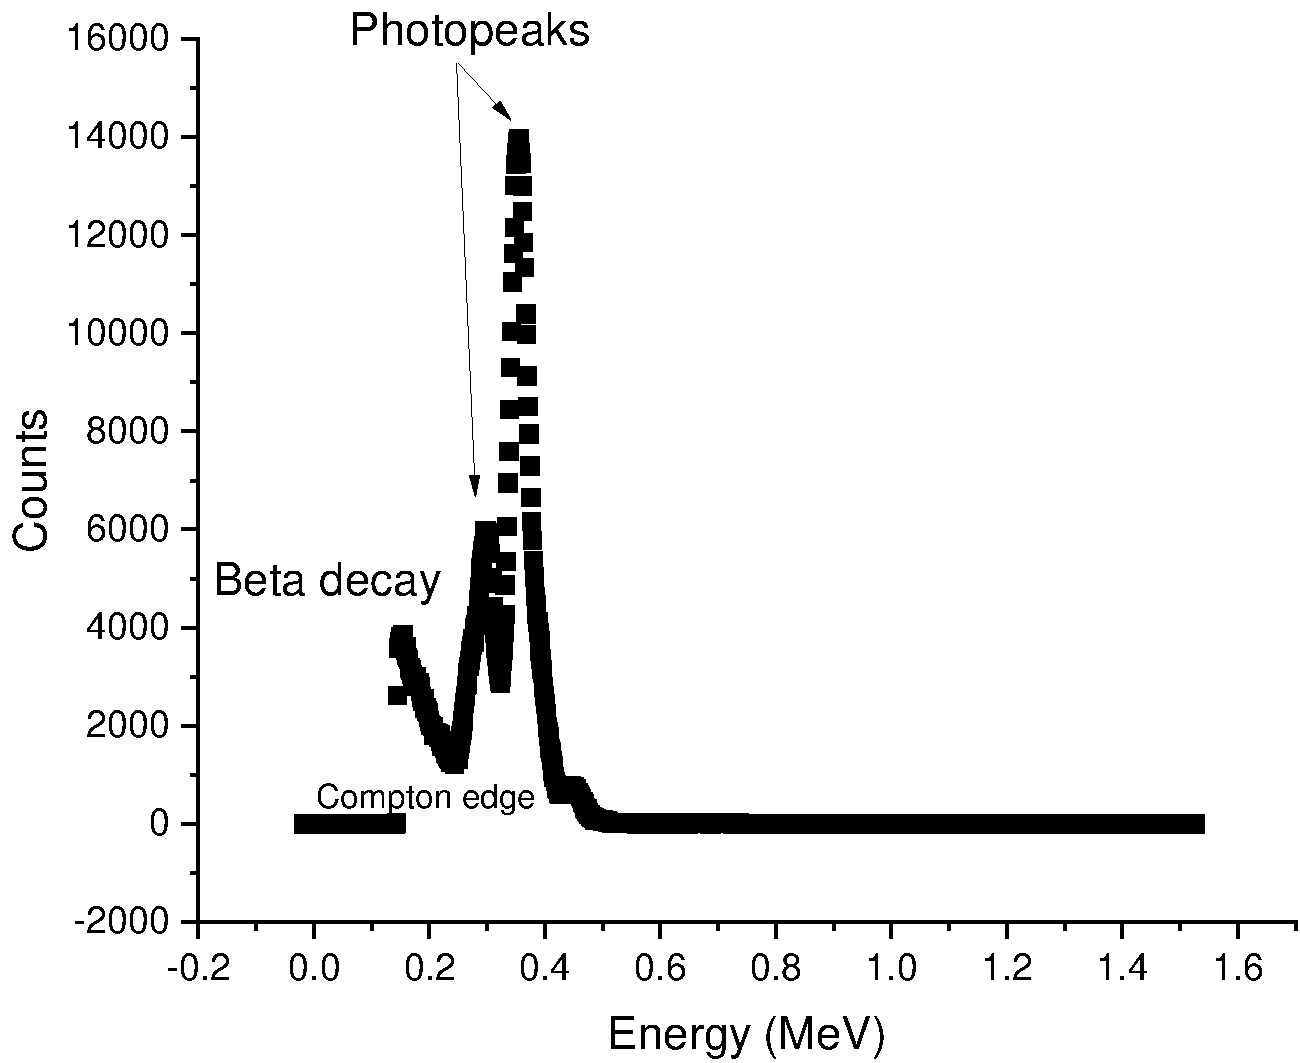
\includegraphics[width=0.7\linewidth]{ba138}
	\caption{Barium-138 spectrum, 608 seconds.}
	\label{fig:ba138}
\end{figure}
\end{document}